\section[Introdução]{Introdução}

  O Hangy nasce da lacuna existente entre as conexões digitais e os encontros presenciais
espontâneos. O mercado atual de aplicativos sociais está saturado de soluções voltadas a
relacionamentos românticos, interações puramente virtuais ou eventos de grande porte que exigem
alto planejamento, o que dificulta a organização de atividades informais e rápidas entre pessoas
com interesses em comum e gera dependência de grupos de mensagens fragmentados. Em paralelo,
estabelecimentos comerciais locais carecem de canais dinâmicos para atrair público de forma
orgânica e em tempo real. A plataforma busca resolver essa dor dupla: fomentar interações
presenciais mais naturais e imediatas para os usuários e, ao mesmo tempo, criar um novo vetor de
atração de clientes para o comércio local, viabilizando um modelo de negócios escalável.
  O projeto conta com uma equipe de 17 estudantes da \ac{pucrs}, em diferentes áreas do curso e com
diferentes conhecimentos, orientados pelo professor Edson Ifarraguirre Moreno.

\begin{figure}[H]
    \centering
    \small
    \caption{Time do Projeto Hangy}
    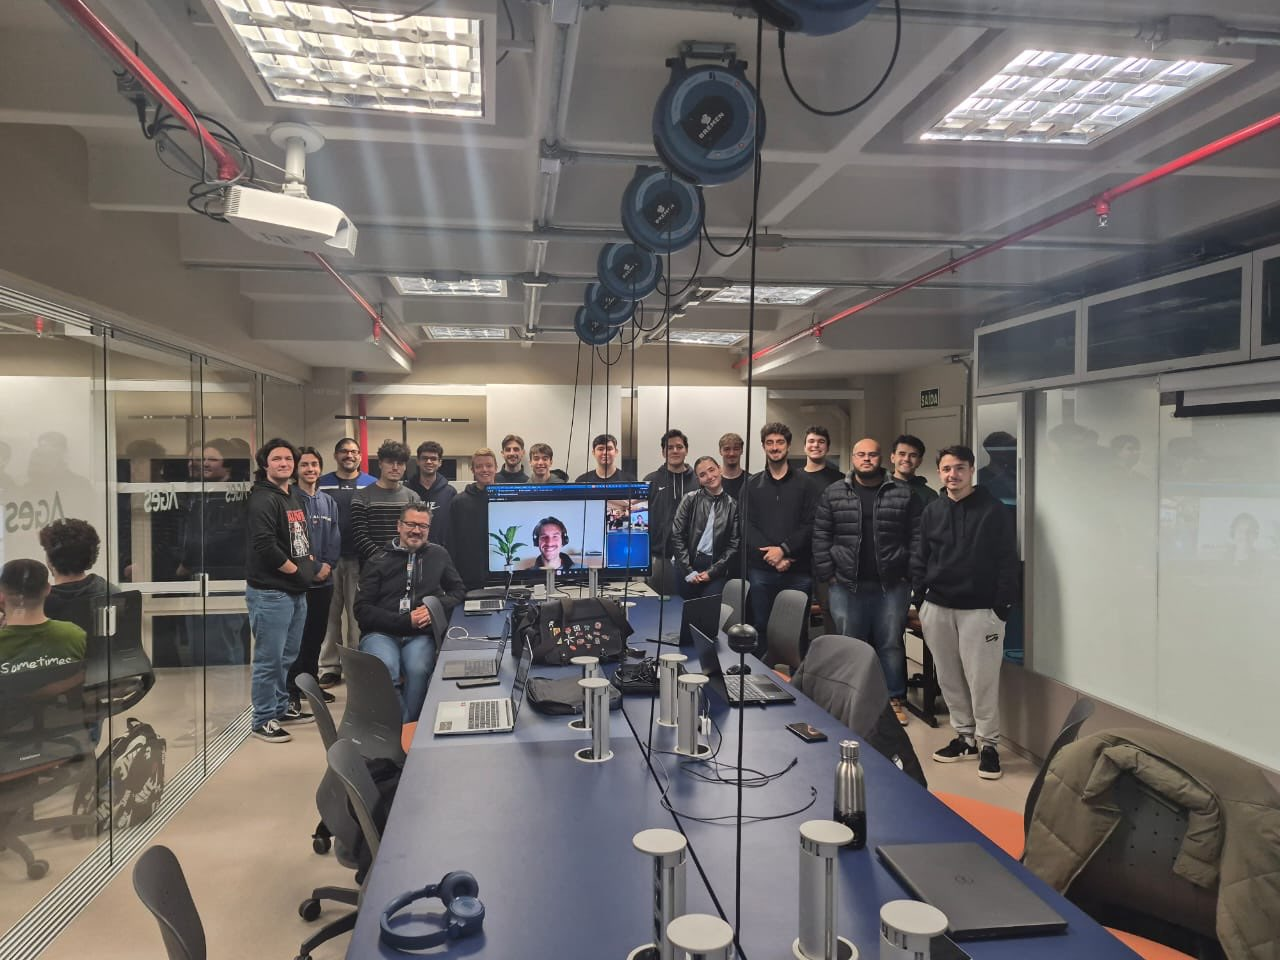
\includegraphics[width=1\linewidth]{conteudo//5 - ages IV//conteudo//figures/hangy-time.png}
    \legend{Fonte: Wiki do projeto}
    \label{fig:projeto-time-hangy}
\end{figure}
